\documentclass[fontsize=11pt]{scrartcl}
%-------------------------------------------------------------------------------------------------
% LATEX TEMPLATE FOR A BACHELOR'S THESIS AT GHENT UNIVERSITY GLOBAL CAMPUS
% CREATED BY MANVEL GASPARYAN
% APRIL, 2021
%-------------------------------------------------------------------------------------------------
\usepackage{hyperref, tikz, float, subfigure, multicol, amsmath, amsthm, alphalph, amsfonts, amssymb, geometry, enumitem, parskip, xcolor, sectsty}
\usepackage[normalem]{ulem}
\usepackage[font=scriptsize,labelfont=bf]{caption}
\usepackage[explicit]{titlesec}
\usepackage[scaled]{helvet}
\renewcommand\familydefault{\sfdefault} 
\usepackage[T1]{fontenc}

\usepackage{setspace}

\usepackage{{listings}}

%-------------------------------------------------------------------------------------------------
 \geometry{a4paper, total={170mm,257mm}, left=20mm, right=20mm, top=25mm, bottom=30mm}
%-------------------------------------------------------------------------------------------------
\newtheorem{proposition}{Proposition}[section]
\newtheorem{lemma}{Lemma}[section]
\newtheorem{remark}{Remark}[section]
\newtheorem{corollary}{Corollary}[section]
\newtheorem{definition}{Definition}[section]
%-------------------------------------------------------------------------------------------------
\pagenumbering{roman}
\usepackage{fancyhdr}
\pagestyle{fancy}
\fancyhf{}
\renewcommand{\headrulewidth}{0pt}
\rhead{}
\lhead{}
\rfoot{\thepage}
\lfoot{}

%-------------------------------------------------------------------------------------------------
\definecolor{ghent_blue}{rgb}{0.1176, 0.392, 0.7843}
\definecolor{ghent_dark}{rgb}{0.0, 0.2, 0.4}
%-------------------------------------------------------------------------------------------------
\title{{\color{ghent_blue} TITLE: LATEX TEMPLATE FOR A BACHELOR'S THESIS AT GHENT UNIVERSITY GLOBAL CAMPUS}}
\subtitle{{\color{ghent_dark} [DOCUMENT SUBTITLE]}}
\date{}         
%-------------------------------------------------------------------------------------------------
\sectionfont{\fontsize{16}{15}\selectfont}
\sectionfont{\color{ghent_blue}}
%=================================================================================================
\begin{document}
%=================================================================================================
%PAGE i: TITLE PAGE 1
%-------------------------------------------------------------------------------------------------
\thispagestyle{empty}
\hfill
\includegraphics[scale = 1]{img/badge/2021.png}\\
%-------------------------------------------------------------------------------------------------
\vspace{8cm}

\noindent{\fontsize{30}{50}\selectfont{\color{ghent_blue}\noindent \hspace{12mm}\textbf{
Microphotonics %TITLE
}}}\\
\fontsize{20}{50}\selectfont{\color{ghent_dark}\noindent \hspace{13mm}\textbf{
CAD-LAB: WAVEGUIDES%SUBTITLE
}}\vspace{10mm}

\hspace{10mm}{\fontsize{10}{10}\selectfont{\textbf{
Lukuan Zhang, Rui Zhu, Xiyuan Guo%AUTHOR
}}}
\vspace*{\fill}
%-------------------------------------------------------------------------------------------------
\begin{flushleft}
\begin{figure}[b!]

\includegraphics[scale = 1.4]{img/badge/GUGC.pdf}
\end{figure}
\end{flushleft}

\doublespacing
\tableofcontents
\pagebreak
\pagenumbering{arabic}

%=================================================================================================
%TASK 1
%-------------------------------------------------------------------------------------------------
\section{\uline{Reducing the 3D structure to 2D: the effective index method}}
%-------------------------------------------------------------------------------------------------
% Here comes some text. This text makes use of 1.5 line spacing. 
%-------------------------------------------------------------------------------------------------
\subsection{}
%-------------------------------------------------------------------------------------------------
By simulating the slab waveguide modes, we get the fundamental TE-mode with,
\begin{equation} 
    n_{core}=2.855119 
    \label{eq1}
\end{equation}
Comparing those modes, we find the least transmission when
\begin{equation} 
    n_{cladding}=1.527117 
    \label{eq2}
\end{equation}
%-------------------------------------------------------------------------------------------------
\subsection{}
%-------------------------------------------------------------------------------------------------
From the bend coupler we get $\beta=2.60528$
%-------------------------------------------------------------------------------------------------
\subsection{Observation}
%-------------------------------------------------------------------------------------------------
\textbf{Fundamental mode:} As Figure \ref{fig1.1} shown, 
the results are almost the same in the center of the core. 
But the boudary shows the different effects. 
The actual TE-mode exists one small peak each side, but the slab-mode not.
\begin{figure}[H]
    \centering
     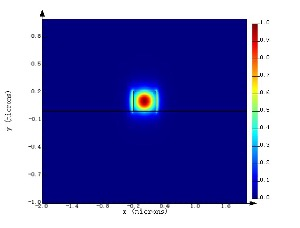
\includegraphics[width=0.45\textwidth]{img/fig1.1a.jpg} % set width to get a proper ratio
     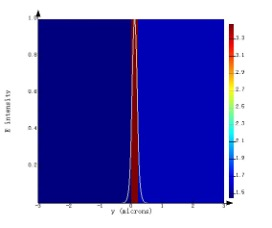
\includegraphics[width=0.45\textwidth]{img/fig1.1b.jpg}
     \caption{Fundamental mode: actual TE-mode (left); 2D slab TE-mode (right)}
     \label{fig1.1}
\end{figure}
\textbf{Modes on the two interface:} They show a quite similar results in Fig \ref{fig1.2}.
\begin{figure}[H]
    \centering
     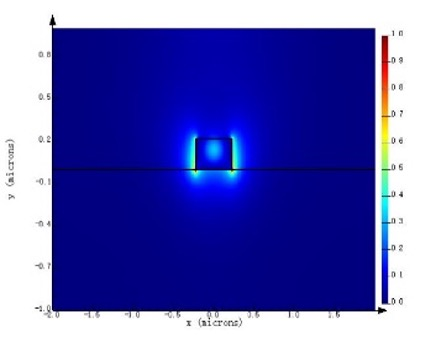
\includegraphics[width=0.45\textwidth]{img/fig1.2a.jpg} % set width to get a proper ratio
     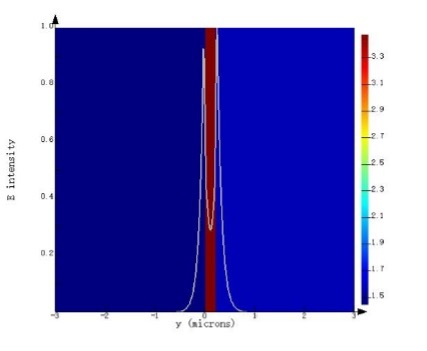
\includegraphics[width=0.45\textwidth]{img/fig1.2b.jpg}
     \caption{Mode on interface: actual TE-mode (left); 2D slab TE-mode (right)}
     \label{fig1.2}
\end{figure} 
\textbf{Other modes:} It is difficult to find some similarities among them.
\textbf{The validity of the effective index method:}
It is available when studing the fundamental mode of the center 
(or ignoring the boundary effect), or studying the interface mode.
%=================================================================================================
\pagebreak
%=================================================================================================
%TASK 2
%-------------------------------------------------------------------------------------------------
\section{\uline{Waveguide-ring coupler}}
%-------------------------------------------------------------------------------------------------
% Here comes some text. This text makes use of 1.5 line spacing. 
%-------------------------------------------------------------------------------------------------
\subsection{}
%-------------------------------------------------------------------------------------------------
The Fig \ref{fig2.1} shows how the light propagates through the coupler and partly couples 
to the bent waveguide. 
\begin{figure}[H]
    \centering
     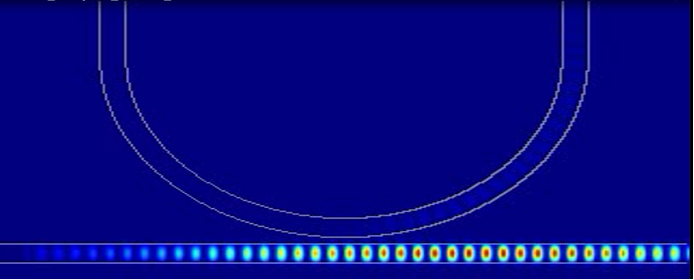
\includegraphics[width=0.7\textwidth]{img/fig2.1.png}
     \caption{Here to write the caption of the figure.}
     \label{fig2.1}
\end{figure} 
%-------------------------------------------------------------------------------------------------
\subsection{}
%-------------------------------------------------------------------------------------------------
With a continuous wave input,
the behavior of the splitter is shown in figure \ref{fig2.2}.
The first row is linear,
and the second row is the logarithmic.
It is obvious that the coupler is not very wavelength-dependent.
\begin{figure}[H]
    \centering
     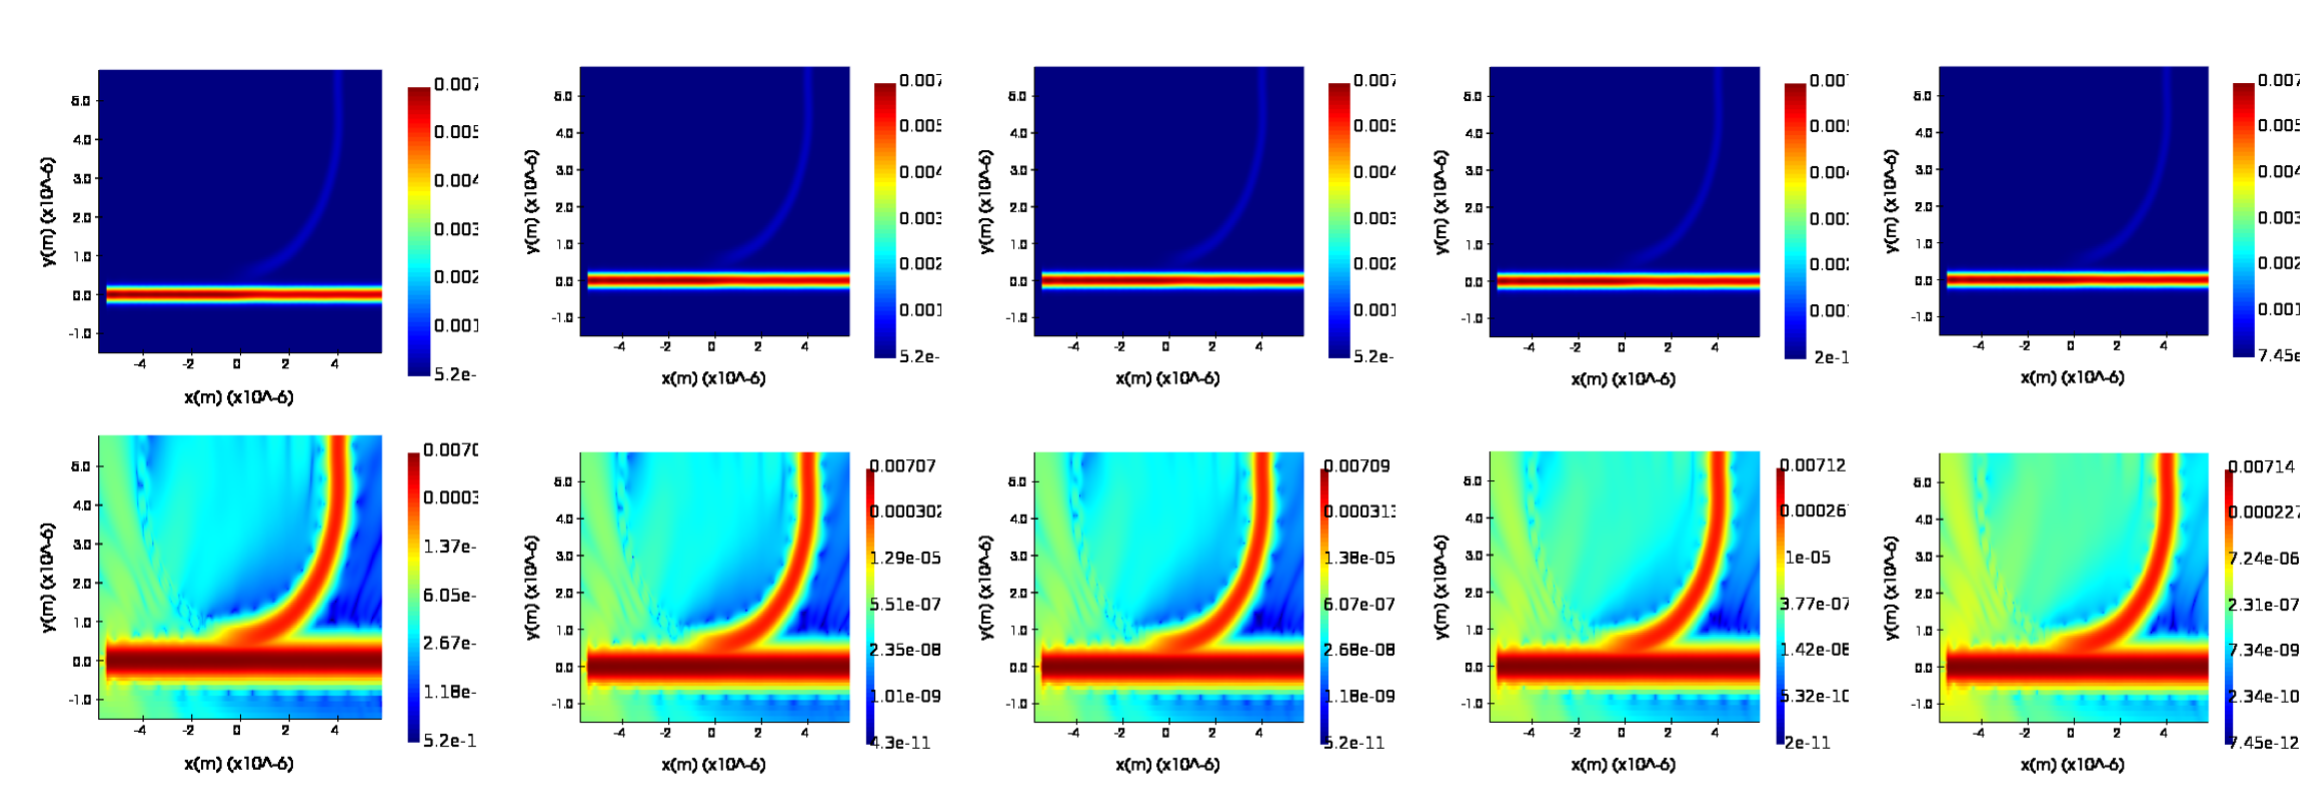
\includegraphics[width=1\textwidth]{img/fig2.2.png}
     \caption{Here to write the caption of the figure.}
     \label{fig2.2}
\end{figure} 
%-------------------------------------------------------------------------------------------------
\subsection{}
%-------------------------------------------------------------------------------------------------
Fig \ref{fig2.3} shows the trasmission factor $r$, rises at three different ring-radius 
as the gap distance increases. The changing trend of them are similar 
as $r$ and gap distance is positively correlated. It can be seen that 
$r$ and gap-distance is linear positive correlation.
\begin{figure}[H]
    \centering
     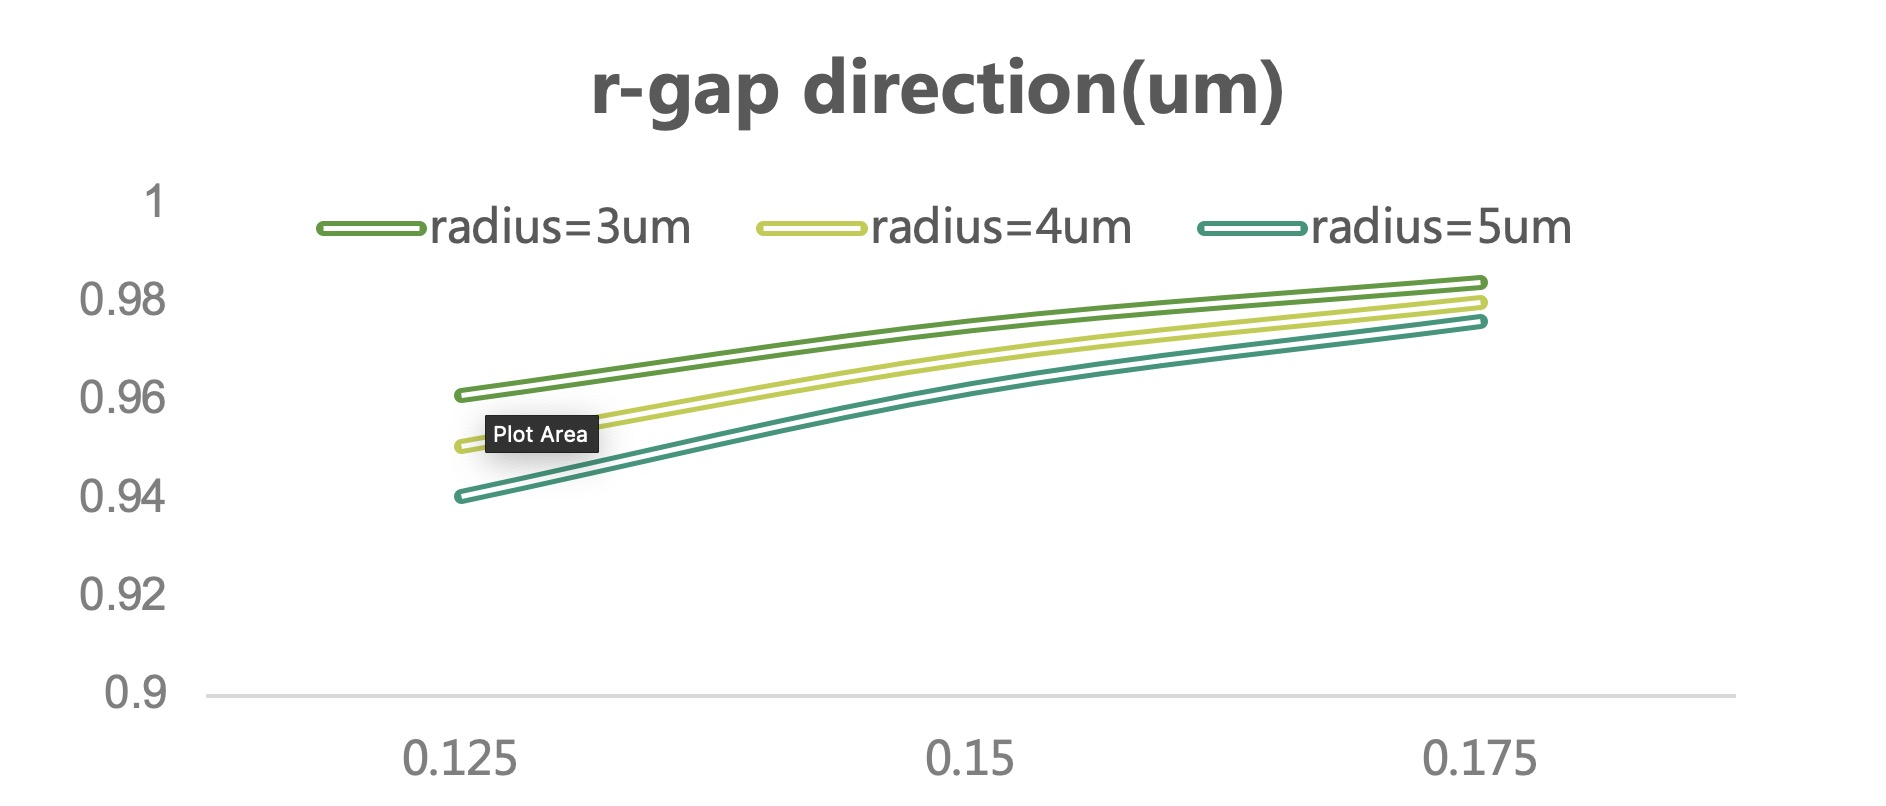
\includegraphics[width=0.7\textwidth]{img/fig2.3.png}
     \caption{Here to write the caption of the figure.}
     \label{fig2.3}
\end{figure} 
%=================================================================================================
\pagebreak
%=================================================================================================
%TASK 3
%-------------------------------------------------------------------------------------------------
\section{\uline{Add-drop filter}}
%-------------------------------------------------------------------------------------------------
% Here comes some text. This text makes use of 1.5 line spacing. 
%-------------------------------------------------------------------------------------------------
\subsection{}
%-------------------------------------------------------------------------------------------------
There is three $\lambda_{res}$, $1569.32nm$, $1538.01nm$ and $1507.83nm$, which is related to 
the T distribution of dft\_wg\_output. The average FSR of two initial FSR is $30.745nm$, with 
\begin{equation} 
    FSR =  \frac{\lambda ^{2} }{n_gL}, n_g=3.109
    \label{eq3}
\end{equation}
\begin{figure}[H]
    \centering
     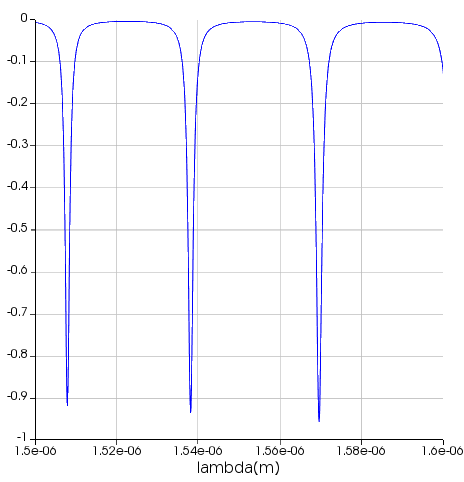
\includegraphics[width=0.5\textwidth]{img/fig3.1.png}
     \caption{Here to write the caption of the figure.}
     \label{fig3.1}
\end{figure} 
%-------------------------------------------------------------------------------------------------
\subsection{}
%-------------------------------------------------------------------------------------------------
When educing the waveguide range to $[1530nm,1550nm]$, 
T distribution of dft\_wg\_output is shown in Fig \ref{fig3.2}, 
$\lambda_{res}=1538.03nm$. 
T of dft\_wg\_output in bend\_coupler.fsp at $\lambda_{res}$ is $0.905347$. 
For $n_g=3.109$, the FWHM can be calculated by 
\begin{equation}
    \mathrm{FWHM}=\frac{\left(1-r^{2}\right) \lambda^{2} r e s}{\pi n g L r}
    \label{eq4}
\end{equation}
and finally we get $FWHM=958.6pm$.
\begin{figure}[H]
    \centering
     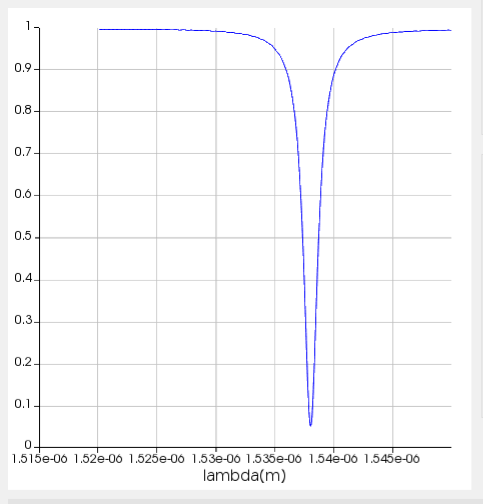
\includegraphics[width=0.5\textwidth]{img/fig3.2.png}
     \caption{Here to write the caption of the figure.}
     \label{fig3.2}
\end{figure}  
%-------------------------------------------------------------------------------------------------
\subsection{}
%-------------------------------------------------------------------------------------------------
% Here comes some text. This text makes use of 1.5 line spacing. 

%=================================================================================================
\pagebreak

%=================================================================================================
%Appendix A
%-------------------------------------------------------------------------------------------------
% \section*{\uline{APPENDIX A}}
% %-------------------------------------------------------------------------------------------------
% Here comes some text. This text makes use of 1.5 line spacing. %=================================================================================================
% \pagebreak
%=================================================================================================
% %Appendix B
% %-------------------------------------------------------------------------------------------------
% \section*{\uline{APPENDIX B}}
% %-------------------------------------------------------------------------------------------------
% Here comes some text. This text makes use of 1.5 line spacing.\\
% In order to cite use \cite{Bern:1}, \cite{Bez:1}, \cite{BioModels}, \cite{Row:1} %=================================================================================================
% \pagebreak
% %=================================================================================================
% \bibliographystyle{plain}
% \bibliography{References}
%=================================================================================================

\end{document}